\section{Architecture and Implementation}


The architecture of the safety annex plugin is shown in Figure~\ref{fig:plugin-arch}.  It is written in Java and is hosted in the OSATE AADL toolset, which is in turn built on Eclipse.  It is not designed as a stand-alone extension of the language, but to work with existing behavioral information in the {\em Assume-Guarantee Reasoning Environment} (AGREE) AADL annex and tools~\cite{NFM2012:CoGaMiWhLaLu}.  AGREE allows {\em assume-guarantee} behavioral contracts to be added to AADL components.  The language used for contract specification is based on the LUSTRE dataflow language~\cite{Halbwachs91:IEEE}. The tool allows scaling of formal verification to large systems by splitting the analysis of a complex system architecture into a collection of verification tasks that correspond to the structure of the architecture.

\begin{figure}
\begin{center}
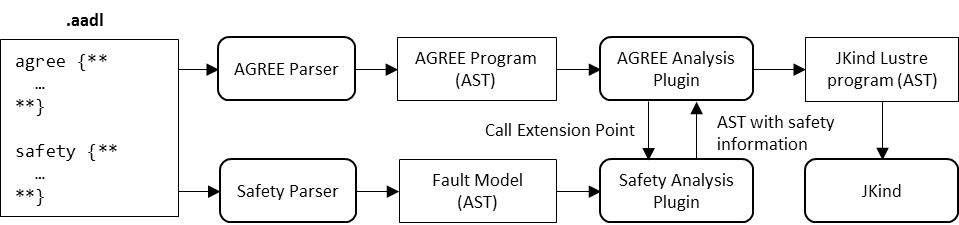
\includegraphics[trim=0 400 430 0,clip,width=0.85\textwidth]{images/arch.png}
\end{center}
\vspace{-0.2in}
\caption{Safety Annex Plug-in Architecture}
\label{fig:plugin-arch}
\end{figure}

AGREE contracts are normally used to define the nominal behaviors of system components as {\em guarantees} under {\em assumptions} about the values the component's environment will provide.  The safety annex extends these contracts to allow faults to modify the expected behavior of component inputs and outputs.  To allow for these kinds of extensions, AGREE implements an Eclipse extension point interface that allows other plug-ins to modify the generated AST prior to its submission to the solver.  If the safety annex is enabled, these faults are added to the AGREE contract and, when activated, override the normal guarantees provided by the component.  An example of a portion of an initial AGREE node and its extended contract is shown in Figure~\ref{fig:comp}.  The \texttt{\_\_fault} variables and declarations are added to allow the contract to override the nominal behavioral constraints (provided by guarantees) on outputs.  In the Lustre language, \texttt{assertion}s are constraints that are assumed to hold in the transition system.

\begin{figure}
\vspace{-0.1in}
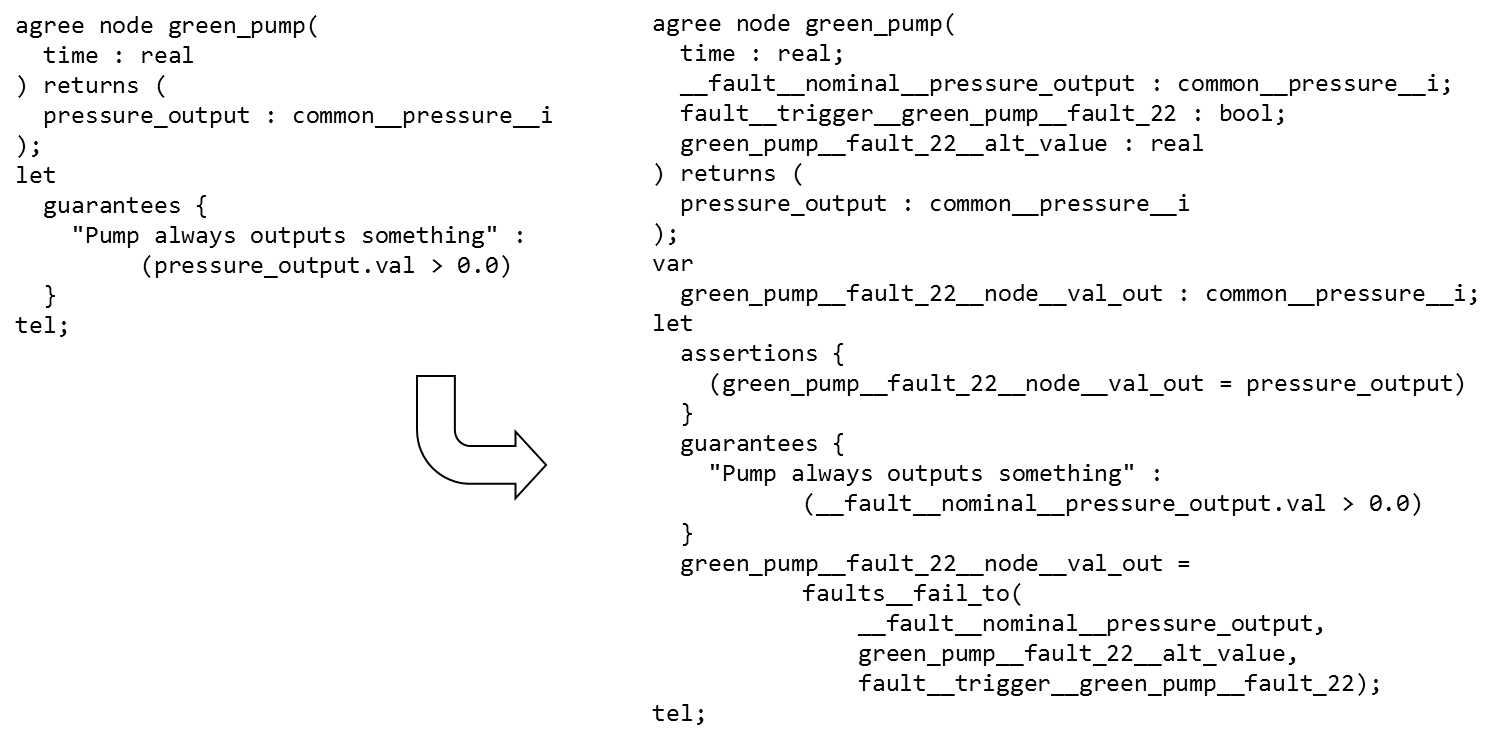
\includegraphics[trim=30 150 120 10,clip,width=\textwidth]{images/sample_code.png}
\vspace{-0.3in}
\caption{Nominal AGREE node and its extension with faults}
\label{fig:comp}
\end{figure}

An annotation in the AADL model determines the fault hypothesis: either that a maximal number of faults can be active at any point in execution (often one or two), or that only faults whose probability of simultaneous occurrence is above some probability threshold.  In the former case, we assert that the sum of the 'true' {\em fault\_\_trigger} variables is under some integer threshold.  In the latter, we determine all fault combinations of faults whose probabilities are above the specified probability threshold, and describe this as a proposition over {\em fault\_\_trigger} variables.

Once augmented with safety information, the AGREE model follows the standard AGREE translation path to the model checker JKind~\cite{2017arXiv171201222G}, an infinite-state model checker for safety properties.  The augmentation includes traceability information so that when counterexamples are displayed to users, the active faults for each component are visualized.



